\documentclass[11pt, aspectratio=169]{beamer}
\usepackage[utf8x,utf8]{inputenc}
\usepackage[ngerman]{babel}

\newcommand{\Title}{Zusammenfassung: \\ Harmonizing Company Wide Information Objects \\ }
\newcommand{\Subtitle}{Alexander Schmidt, Dr. Boris Otto}
\newcommand{\TitleFooter}{Zusammenfassung: Harmonizing Company Wide Information Objects}
\newcommand{\ReferentIn}{Aleksandar Topic}
\newcommand{\Matrikelnummer}{(677502)}
\newcommand{\Picture}{
\includegraphics[width=2cm]{./@Bilder/at.jpeg}}
\date{08.01.2024}

% Schriftsatz
\usepackage{fontawesome5}
\usepackage[scaled]{helvet}
\renewcommand\familydefault{\sfdefault}
\usepackage{metalogo}

% Mathematische Zeichen
\usepackage{amsmath}
\usepackage{amsfonts}
\usepackage{amssymb}

% Grafiken einbinden
\usepackage{graphicx}
\usepackage{pdfpages}

% TikZ und Datenanalyse
\usepackage{pgfplotstable}
\pgfplotsset{compat=newest, compat/bar nodes=1.8}
\usetikzlibrary{shadows, fadings, decorations, decorations.text, arrows, arrows.meta, patterns, shapes.geometric}
\usetikzlibrary{decorations}
\usepgflibrary{arrows}
\usetikzlibrary{arrows}
\usetikzlibrary{patterns}

% UML-Package
\usepackage{pgf-umlcd}

% TikZ-Grafiken einbetten
\newcommand{\TikZGraphic}[1]{
  \begin{center}{\fontsize{6}{-4}\fontfamily{phv}\fontshape{sl}\selectfont \setlength{\unitlength}{1.0pt}
    \begin{tikzpicture}[scale=1.0, thick]\input{#1}\end{tikzpicture}
  }\end{center}
}
\newcommand{\tiktxt}[4]{ % [1]: x-Position, [2]: y-Position, [3]: Breite des Textfeldes, [4]: Text
  \draw(#1 mm,#2 mm) node {\begin{minipage}{#3 mm}\begin{center}\setlength{\baselineskip}{2.5ex} #4\end{center}\end{minipage}};
}
\newcommand{\rtiktxt}[5]{ % [1]: x-Position, [2]: y-Position, [3]: Breite des Textfeldes, [4]: Text, [5]: Winkel für die Rotation
  \draw(#1 mm,#2 mm) node[rotate=#5] {\begin{minipage}{#3 mm}\begin{center}\setlength{\baselineskip}{2.5ex} #4\end{center}\end{minipage}};
}

% Farbpakete und eigene Farben
\usepackage{xcolor}
\usepackage{colortbl}
\usepackage{tcolorbox}
\definecolor{color1}{HTML}{073c60}		% Dunkles Blau (Hochschulblau)
\definecolor{color2}{HTML}{333333}		% Dunkles Grau (für Überschriften)
\definecolor{color3}{HTML}{7592ad}		% Helles Blau
\definecolor{color4}{HTML}{e3e9ed}		% Sehr helles Blau
\definecolor{color5}{HTML}{c1c8d6}		% helles Blaugrau
\definecolor{linkcolor}{HTML}{073c60}	% Farbe für Links

% Schreibabkürzung
\newcommand{\lb}{\linebreak} 
\newcommand{\high}[1]{\textcolor{color1}{\textbf{#1}}}

% Metaangaben zum Vortrag übertragen
\title{\Title}
\subtitle{\Subtitle}
\author{\ReferentIn~\Matrikelnummer}
\institute{Hochschule Worms}
\logo{}

% Externe Links, klickbare URLs
\usepackage{url}
\usepackage{hyperref}
\hypersetup{
    colorlinks,
    linkcolor={color1},
    citecolor={color1},
    urlcolor={linkcolor},
    pdfborderstyle={/S/U/W 1}
}
\usepackage{qrcode}

% Literaturverwaltung und rechtsbündige Quellenangaben
\usepackage{natbib}
\newcommand{\tocite}[1]{\hfill\tiny #1}

% Boxen für Definitionen, die dann farblich im Text hervorgehoben werden
\def\fullboxbegin{\begin{tcolorbox}[colback=color4,colframe=color3,coltext=color1,arc=0mm,boxrule=1pt]}
\def\fullboxend{\end{tcolorbox}}

% Einstellungen für Beamer
\usetheme{Bergen}
\beamertemplatenavigationsymbolsempty					% Keine Navigationszeile am unteren Rand
\setbeamercovered{transparent}							% Einblendeffekt für aufzubauende Grafiken
\def\insertauthorindicator{\faUser}						% Default is "Who?" 
\def\insertinstituteindicator{\faUniversity}			% Default is "From?"
\def\insertdateindicator{\faCalendar*}     				% Default is "When?"
\setbeamercolor{normal text}{fg=color1} 	  			% Textfarbe, normaler Text
\setbeamercolor{title}{fg=color1}						% Dunkelblauer Titel der Präsentation
\setbeamercolor{frametitle}{fg=color1}					% Dunkelblaue Folienüberschrift
\setbeamercolor{description item}{parent=color1}		% Dunkelblauer Text für Description
\setbeamerfont{text}{size=\tiny}						% Schriftgröße auf Folien
\setbeamertemplate{frametitle}{\textbf{\insertframetitle}}		% Schriftart Folienüberschrift
\setbeamerfont * {description item}{series=\bfseries\boldmath}	% Schriftart Description
\setbeamercolor{sidebar}{bg=color1}						% Dunkelblauer Seitenstreifen
\setbeamersize{sidebar width left=21mm}					% Breite Seitenstreifen

% Verschiebe das Inhaltsverzeichnis aus der linken Spalte in die eigentliche Folie
\setbeamertemplate{section in toc}{\inserttocsection}
\setbeamertemplate{subsection in toc}{\inserttocsubsection}
\setbeamertemplate{subsubsection in toc}{\inserttocsubsubsection}

% Neuer Befehl, um eine Folie mit einem Icon versehen zu können
\newcommand{\frametitleNew}[2]{
  \begin{tikzpicture}[remember picture, overlay]
    \node at ([xshift=10.5mm,yshift=-6mm]current page.north west) {\Huge\textcolor{white}{#1}};
  \end{tikzpicture}  
  \frametitle{#2}
}

% Fußzeile und weitere Einstellungen für Folgefolien
\setbeamercolor{footlinecolor}{fg=color1, bg=white}
\defbeamertemplate*{footline}{infolines theme}{
   \leavevmode\hbox{
   	\begin{beamercolorbox}[wd=.15\paperwidth,ht=2.25ex,dp=1ex, left]{white}%
     	{\hspace*{2pt}\ReferentIn}
   \end{beamercolorbox}
   
   \begin{beamercolorbox}[wd=.7\paperwidth,ht=2.25ex,dp=1ex,center]{white}%
     \textcolor{color1}{\insertshortdate{}: \TitleFooter}
   \end{beamercolorbox}
   
   \begin{beamercolorbox}[wd=.15\paperwidth,ht=2.25ex,dp=1ex,right]{white}
     {\insertframenumber{} / \inserttotalframenumber{} \hspace{2ex}}
   \end{beamercolorbox}
   }
}
\setbeamertemplate{footline}[my footline]

% Listings einbinden
% Sourcecode einbinden mit Unterstützung besonderer Befehle
\usepackage{fourier}
\usepackage{listingsutf8}
\lstset{%
  basicstyle=\fontfamily{pcr}\fontseries{m}\fontshape{n}\tiny,
  keywordstyle=\fontfamily{pcr}\fontseries{b}\fontshape{n}\tiny,
  identifierstyle=\fontfamily{pcr}\fontseries{m}\fontshape{n}\tiny,
  commentstyle=\fontfamily{pcr}\fontseries{m}\fontshape{sl}\tiny,
  stringstyle=\color{color1}\fontfamily{pcr}\fontseries{m}\fontshape{n}\tiny,
  %
  showstringspaces=false,
  showspaces=false,
  showtabs=false,
  tab=rightarrowfill,
  tabsize=3,
  extendedchars=true,
  aboveskip=5mm,          % Abstand über Listing
  belowskip=5mm,          % Abstand unter Listing
  keepspaces=true,
  numbers=left,
  numberstyle=\color{white}\tiny,
  stepnumber=1,
  numbersep=13pt,
  numberblanklines=true,
  extendedchars=true,
  breaklines=true,        % Zeilen umbrechen wenn notwendig
  breakautoindent=true,   % Nach dem Zeilenumbruch Zeile einrücken
  postbreak=\space,       % Bei Leerzeichen umbrechen
  backgroundcolor=\color{yellow!20},
  upquote=true,
  literate=
    {Ä}{{\"A}}1
    {Ö}{{\"O}}1
    {Ü}{{\"U}}1
    {ä}{{\"a}}1
    {ö}{{\"o}}1
    {ü}{{\"u}}1
    {ß}{{\ss}}1
}


\lstdefinestyle{inline}{
  basicstyle=\fontfamily{pcr}\fontseries{m}\fontshape{n}\normalsize,
  keywordstyle=\fontfamily{pcr}\fontseries{sb}\fontshape{n}\normalsize,
  identifierstyle=\fontfamily{pcr}\fontseries{m}\fontshape{n}\normalsize,
  commentstyle=\fontfamily{pcr}\fontseries{m}\fontshape{it}\normalsize,
  stringstyle=\color{color1}\fontfamily{pcr}\fontseries{m}\fontshape{n}\normalsize
}






\begin{document}
\begin{frame}
  \begin{tikzpicture}[remember picture, overlay]
    \node at ([xshift=140mm,yshift=33mm]current page.south west) {\Picture};
  \end{tikzpicture}  
  \titlepage
\end{frame}


\begin{frame}[t, fragile]\frametitleNew{\faTasks}{Inhaltsverzeichnis}
  \tableofcontents
\end{frame}



\section{Gegenstand des Papers}

\begin{frame}[t, fragile]
\frametitleNew{\faList}{Gegenstand des Papers}
\only<1>{
  \begin{itemize}
  \item	Entwicklung der METIO-Methode (Method for Establishing Transparency on Information Objects)
  \item Fallstudien
    \begin{itemize}
        \item Multinationaler Automobilhersteller
        \item Nationales europäisches Eisenbahnunternehmen
    \end{itemize}
  \end{itemize}
}

\only<2>{
  \begin{itemize}
  \item Kein Standard zur Harmonisierung, deshalb METIO
  \item Unternehmen vernachlässigen Management ihrer Informationsobjekte komplett
  \end{itemize}
}
\end{frame}

\section{Probleme bei fehlender Harmonisierung}
\begin{frame}[t, fragile]
\frametitleNew{\faList}{Probleme bei fehlender Harmonisierung}
\only<1>{
  \begin{itemize}
  \item Intransparenz der IO (Informationsobjekte)
  \item Unvollständigkeit der IO
  \item Inkorrekte und veraltete Definitionen zu den IO
  \end{itemize}
}
\end{frame}

\section{Folgen dieser Probleme}
\begin{frame}[t, fragile]
\frametitleNew{\faList}{Folgen dieser Probleme}
\only<1>{
  \begin{itemize}
  \item Milde Katastrophen
      \begin{itemize}
      \item Mehrkosten
      \end{itemize}
  \item Schwere Katastrophen
      \begin{itemize}
      \item Homizide
      \end{itemize}
  \end{itemize}
}
\end{frame}

\section{Umriss}
\begin{frame}[t, fragile]
\frametitleNew{\faList}{Umriss}
  \begin{itemize}
  \item METIO wird entwickelt    
  
  \item Fokus: Stammdaten
      \begin{itemize}
      \item Wurzel aller IOs
      \end{itemize}
      
  \item Werkzeug zur Harmonisierung: Metadaten
      \begin{itemize}
      \item Schablone der Stammdaten
      \item BDD (Business Data Dictionary)
      \end{itemize}

  \item Action Research Methode
  \end{itemize}
\end{frame}

\section{Differenzierung BO IO DO}

\begin{frame}[t, fragile]
\frametitleNew{\faImage[regular]}{Differenzierung BO IO DO}

\begin{center}
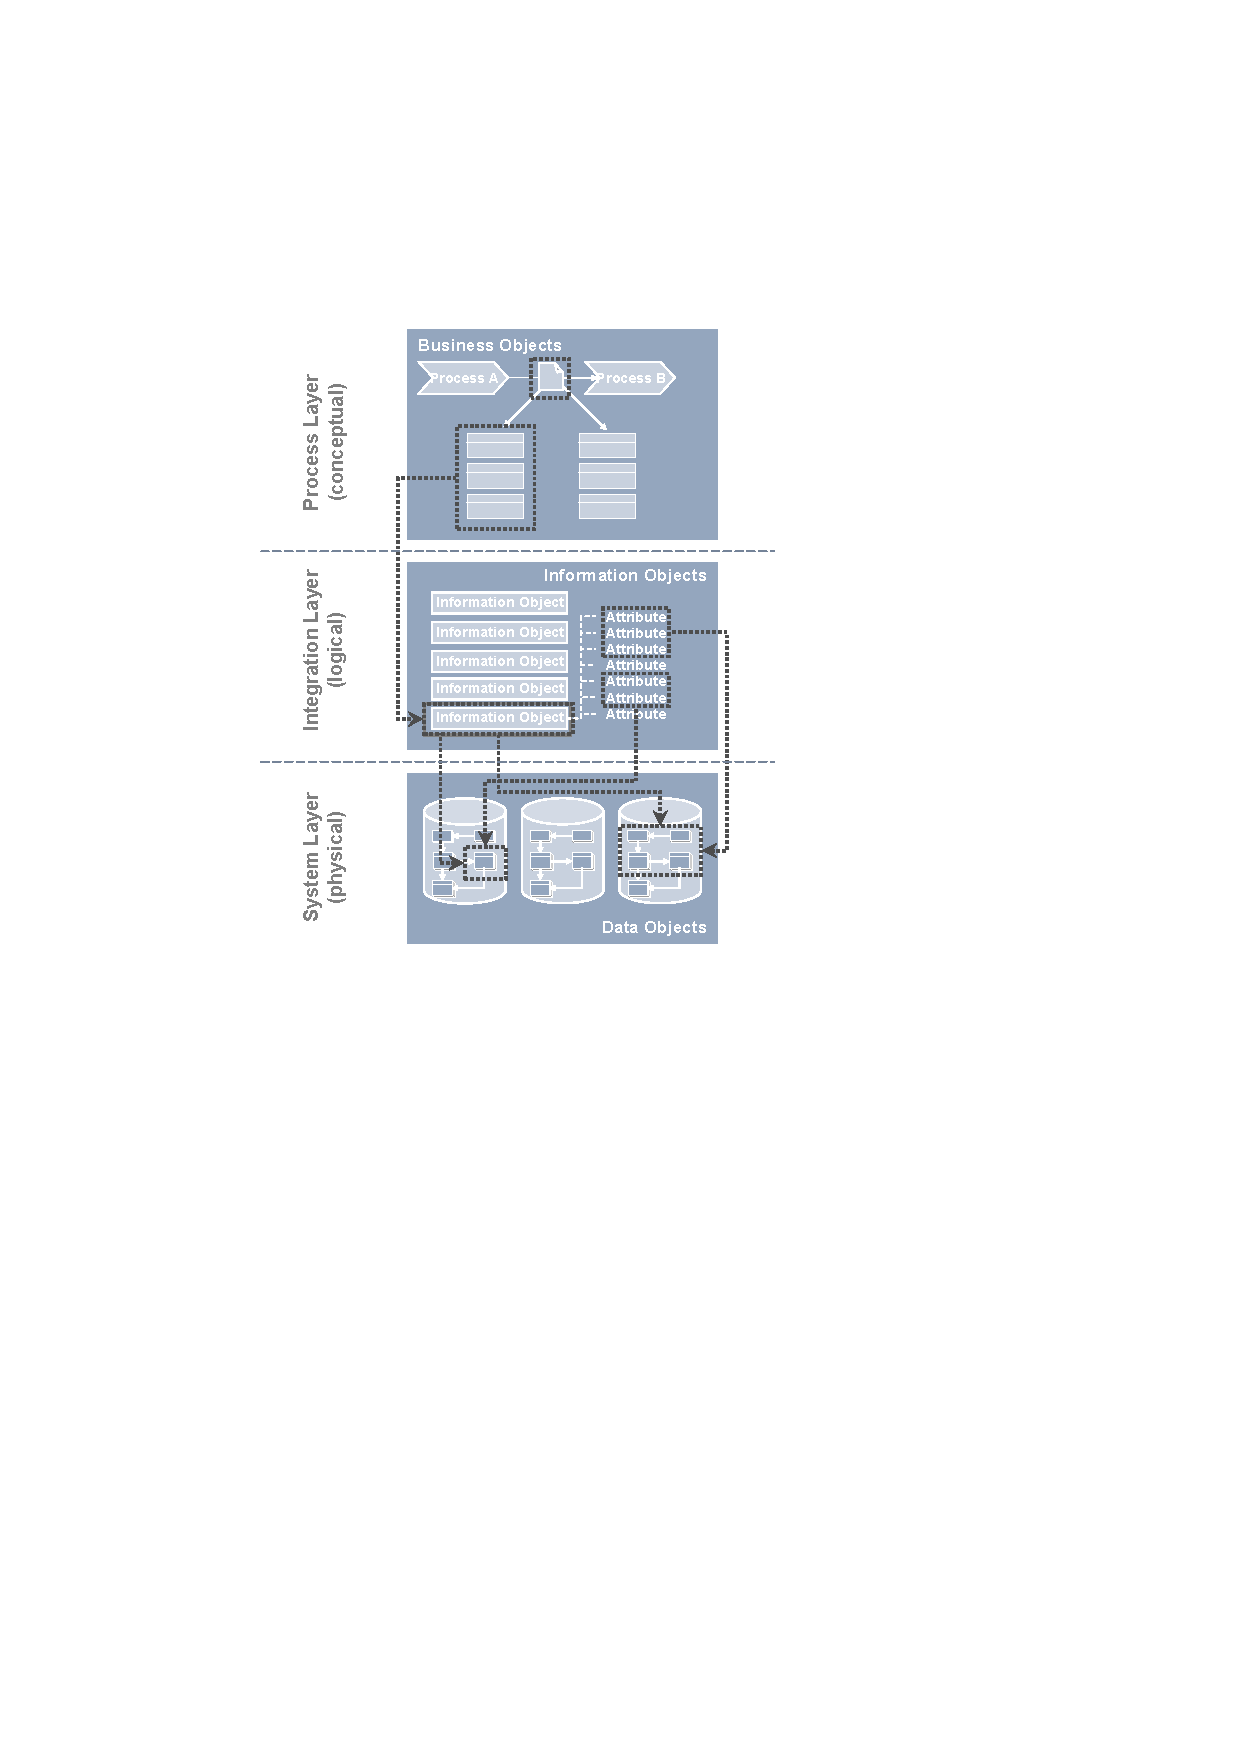
\includegraphics[scale=0.55]{./@Bilder/IOBODO.pdf}

Stammdaten ziehen sich genau durch die drei Ebenen.
\end{center}
\tocite{{\cite{schmidt2008harmonizing}}}
\end{frame}

\section{Ergebnisse}
\begin{frame}[t, fragile]
\frametitleNew{\faPoll}{Ergebnisse}
\only<1>{
  \begin{itemize}
  \item Prozessmodelle
  \item Aktivitätendiagramme
  \item BDD
  \end{itemize}
}
\only<2>{
  \begin{center}
  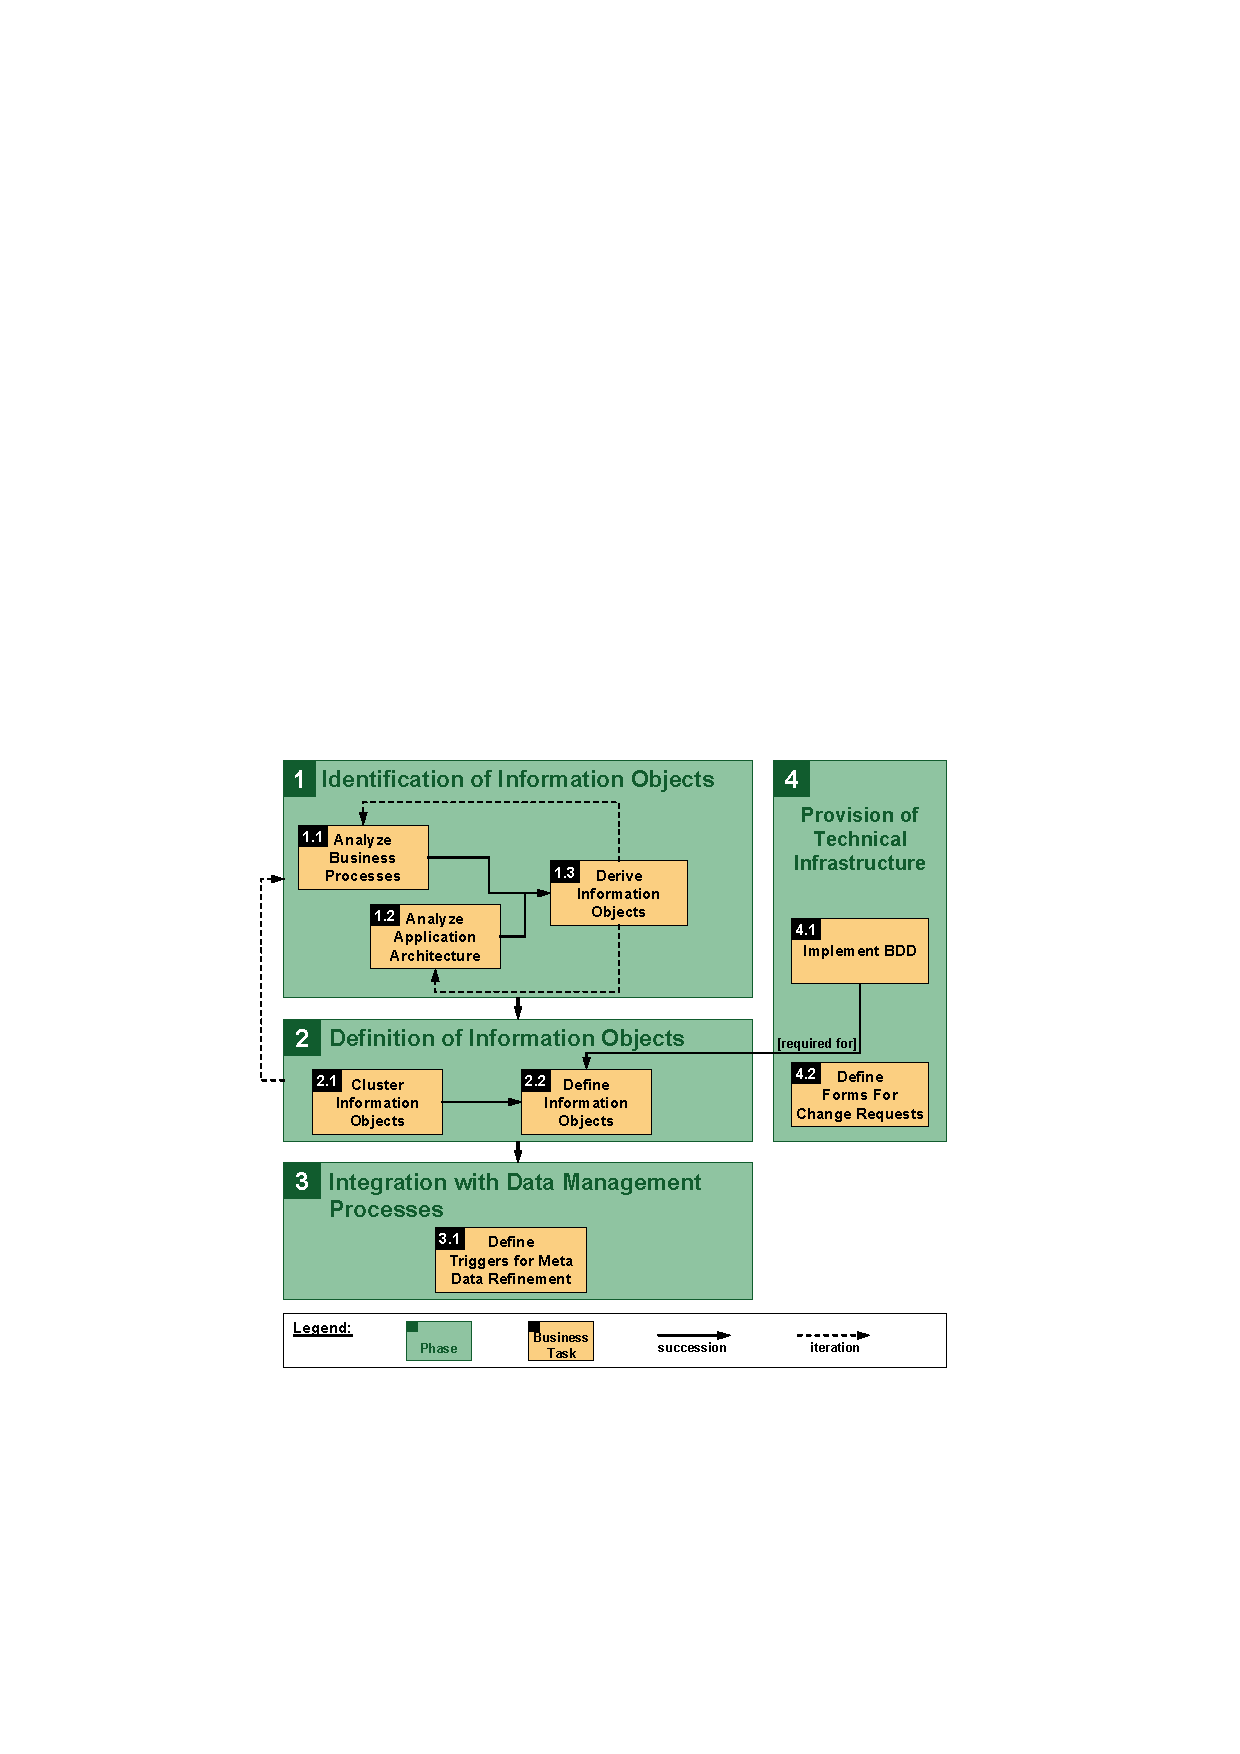
\includegraphics[scale=0.6]{./@Bilder/Prozedur.pdf}
  \end{center}
	
  \tocite{{\cite{schmidt2008harmonizing}}}
}
  \only<3>{
  \begin{center}
  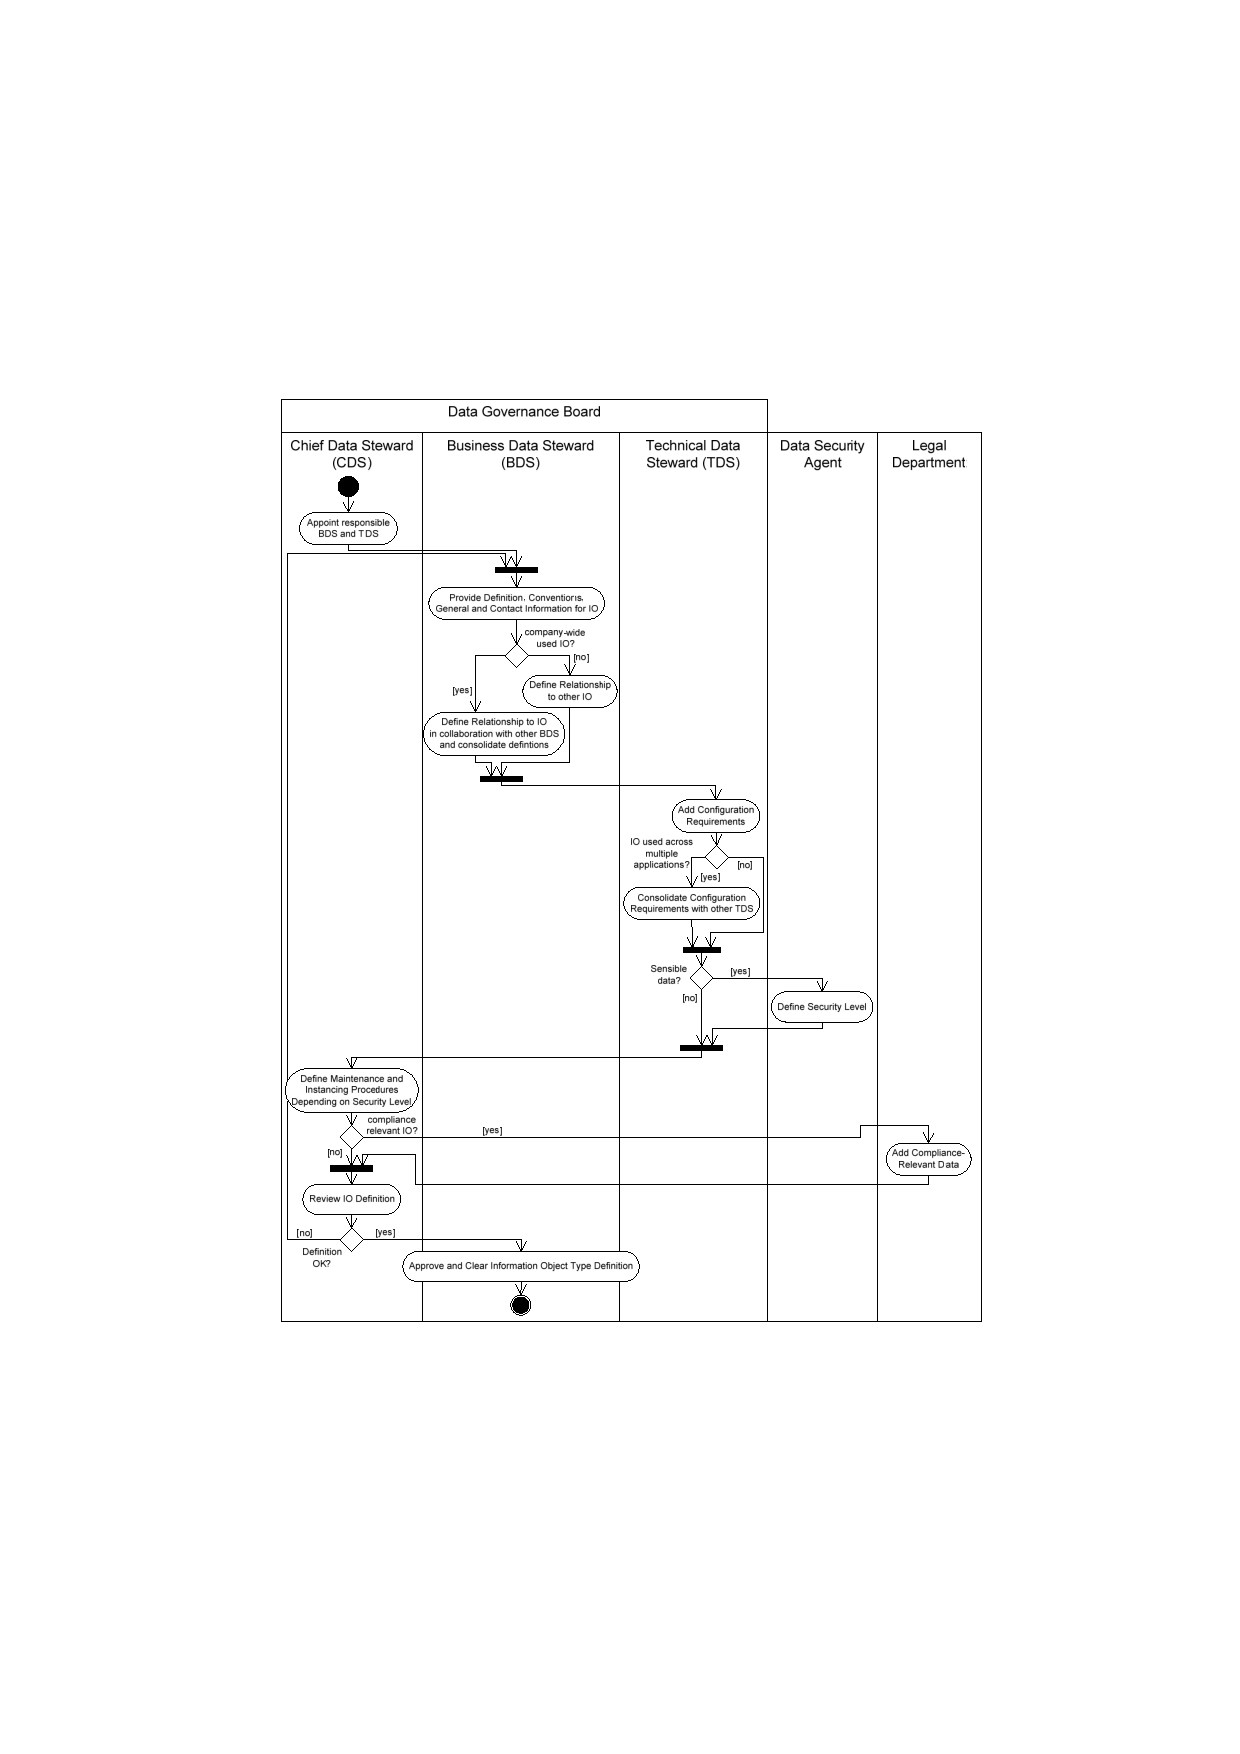
\includegraphics[scale=0.4]{./@Bilder/Akti}
  \end{center}


	
  \tocite{{\cite{schmidt2008harmonizing}}}
}
\only<4>{
  \begin{center}
  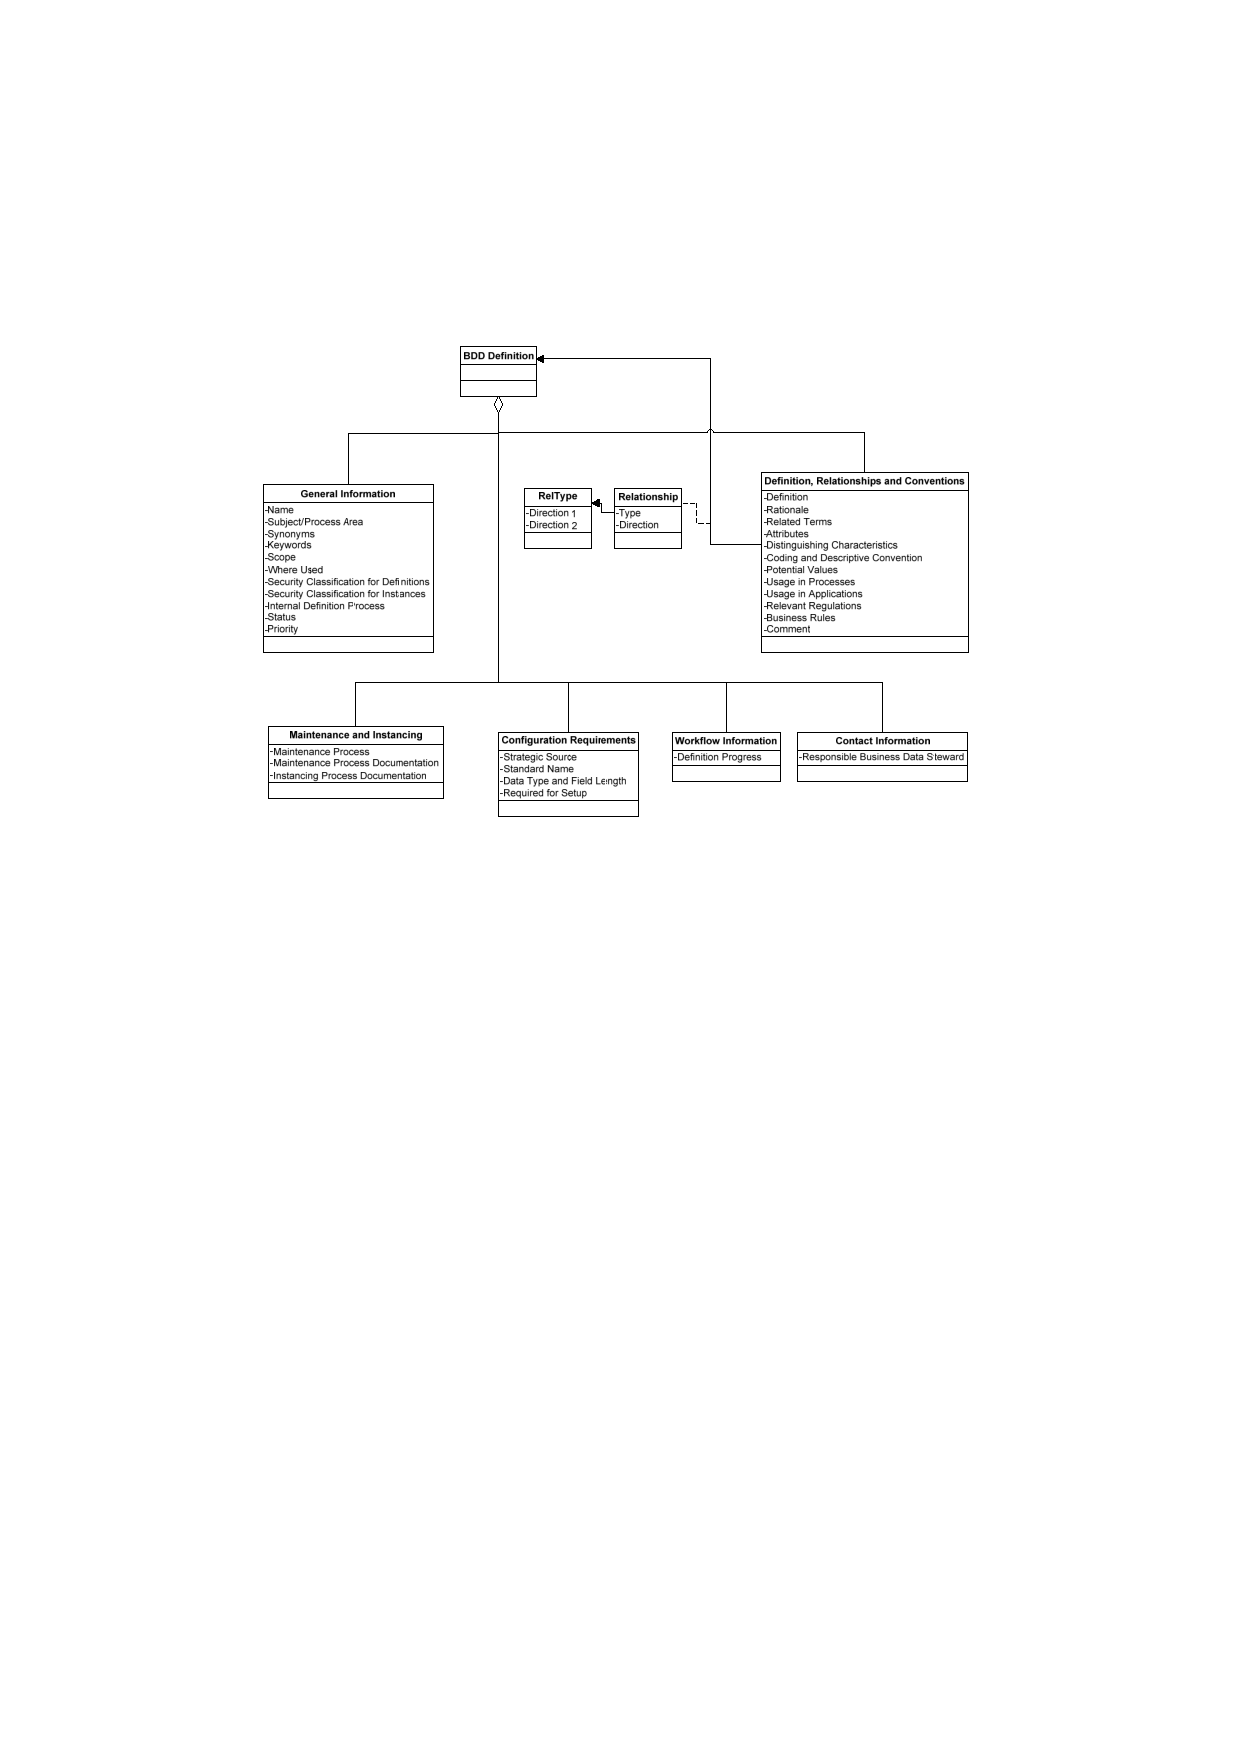
\includegraphics[scale=0.8]{./@Bilder/finalbdd.pdf}
  \end{center}
	
  \tocite{{\cite{schmidt2008harmonizing}}}
}
\end{frame}

\begin{frame}[t, fragile]
\frametitleNew{\faCheck}{}
\begin{center}
Evaluation...
\end{center}
\end{frame}

\begin{frame}[t, fragile]
\frametitleNew{\faSmile}{}
\begin{center}
Danke für die Aufmerksamkeit...
\end{center}
\end{frame}

% Zum Abschluss die bibliographischen Angaben
\frame{\tiny
  \bibliographystyle{hc-de} 
  \bibliography{./@Literatur/literatur}
}
\end{document}
